\section{Introduction}
\begin{wrapfigure}{r}{0.48\textwidth}
  \centering
  \vspace{-18pt}
  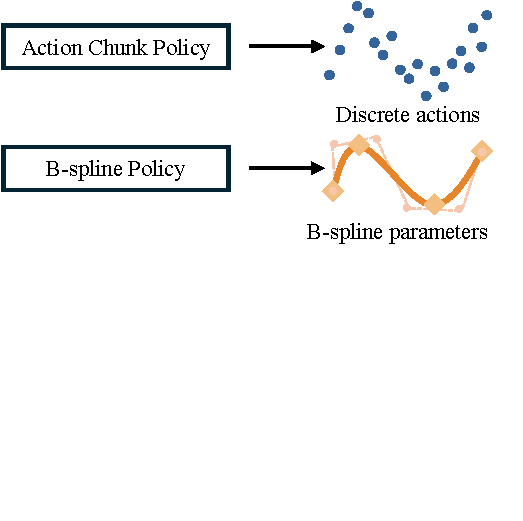
\includegraphics[width=0.46\textwidth]{images/teaser-simple-1.pdf}
  \caption{
  \textbf{\our.} Rather than predicting a chunk of discrete-time actions, \our parameterizes actions as continuous B-spline\protect\footnotemark curves. This continuous representation enables temporal rescaling at execution time, allowing the policy to execute faster and more smoothly.
  }
  \label{fig:teaser-fig}
  \vspace{-10pt}
\end{wrapfigure}
\footnotetext{A B-spline defines a smooth curve by a set of knots and control points. Instead of drawing straight lines between waypoints, a B-spline creates a smooth path that follows their overall trend. Think of it like bending a flexible ruler near waypoints instead of connecting them with sharp corners.}
% version 2
% \begin{wrapfigure}{r}{0.44\textwidth}
%   \centering
%   \vspace{-20pt}
%   \includegraphics[width=0.44\textwidth]{images/teaser-simple-2.png}
%   \caption{
%   \textbf{\our.}
%   \color{red}{Change 3.76}\\
%   Rather than predicting a chunk of discrete-time actions, our \our (BSP) parameterizes actions as continuous B-spline curves defined by a set of knots and control points.
%   Experimental results demonstrate that B-spline representation enables fast robot manipulation, with a large improvement over the baseline method.}
%   \label{fig:teaser-fig}
%   \vspace{-20pt}
% \end{wrapfigure}
% would it be better if we make the figure left to right?
% motivation
% Robotic manipulation through visuomotor policy learning has made remarkable progress in recent years~\cite{pi_05,gr1,act,dp}.
% However,  the speed of task completion remains a major bottleneck.
% Consider the task of folding a t-shirt: while a human typically completes the task in about 10 seconds, even with the most advanced models, robots often require close to a minute.
% This gap poses a critical, unresolved challenge in visuomotor policy learning---\emph{temporal efficiency}: how can a robot quickly complete a task?
Robotic manipulation via visuomotor policy learning has made remarkable progress in recent years~\cite{pi_05,gr1,act,dp}. 
Yet, despite these advances, task execution speed remains a major bottleneck. In everyday manipulation tasks such as folding a T-shirt, humans typically complete the task in roughly 10 seconds, whereas even state-of-the-art robotic systems often require close to a minute~\cite{tshirt, pi_05, black2024pi_0}. This gap exposes a fundamental and largely unresolved challenge in visuomotor policy learning—\emph{efficiency}: how can robots execute complex manipulation tasks quickly, rather than merely complete them successfully?

% One primary source of inefficiency in modern visuomotor policies is the design of their action representations. Most existing approaches represent actions as fixed-length chunks sampled uniformly over time. While chunking can stabilize long-horizon prediction and improve learning performance~\cite{act}, it also imposes inherent limitations.
% %
% First, fixed-length chunking enforces a uniform temporal resolution, implicitly assuming that all phases of a task require the same action granularity. In reality, manipulation tasks have strongly non-uniform temporal structure: rapid motions such as reaching can be executed efficiently with coarse actions, whereas contact-rich phases such as grasping, alignment, and insertion demand fine-grained control.
% %
% Second, executing actions by stitching together independently predicted chunks can introduce discontinuities at chunk boundaries. These artifacts may be tolerable in low-speed or quasi-static regimes, but they become increasingly problematic under fast execution, where boundary mismatches caused by prediction noise or inference latency can lead to jerky motions and degraded performance.

A key source of inefficiency in modern visuomotor policies lies in the design of action chunking~\cite{dp,act}. Most existing approaches parameterize actions as fixed-length chunks sampled uniformly over time. While such chunking can stabilize long-horizon prediction and improve learning performance~\cite{mobile-aloha}, it also introduces inherent limitations: 
\vspace{-5pt}

\begin{itemize}[leftmargin=3mm]
    % \item \textit{Flexible hardware requirements.} 
    \item \textit{Uniform temporal resolution.} 
    Fixed-length chunks assume that every phase of a task requires identical control granularity. In practice, manipulation tasks exhibit strongly non-uniform temporal structure: fast motions such as reaching can be executed rapidly with coarse actions, whereas contact-rich phases such as grasping, alignment, and insertion demand fine-grained precision. Uniform chunking fundamentally misallocates representational capacity across time.
\end{itemize}
\vspace{-5pt}

\begin{itemize}[leftmargin=3mm]
    \item \textit{Chunk discontinuities.} 
    Stitching together independently predicted action chunks at inference time can introduce discontinuities at chunk boundaries. While such boundary mismatches may be tolerable in low-speed or quasi-static settings, they become highly problematic during high-speed execution, where even small errors can lead to tracking failures or complete task failure.
\end{itemize}

% \begin{figure}[t!]
%   \centering
%   \includegraphics[width=0.45\textwidth]{images/teaser-5.pdf}
%   \captionof{figure}{
%   \textbf{\our.}
% Rather than predicting a chunk of discrete-time actions, our \our (BSP) parameterizes actions as continuous B-spline curves defined by a set of knots and control points.
% %
% Experimental results demonstrate that B-spline representation enables fast robot manipulation, with a \textbf{3.76×} improvement over the baseline method.}
% \label{fig:teaser-fig}
% \end{figure}

\vspace{-5pt}
These limitations motivate a paradigm shift: representing robot actions as \emph{\textbf{continuous curves}} rather than discrete waypoint chunks. Such a representation is used in classical motion planning~\cite{to-pnp-with-bsplines,to-via-bsplines,bsplines-based-trajectory-design,bspline-on-gcs} and computer graphics~\cite{bspline-in-cad-cg,intro-bspline-graphics}, where spline-based representations are widely favored for being smooth, compact, and mathematically tractable. Among spline families, B-splines are especially attractive for visuomotor control: they are smooth by construction, provide compact parameterizations~\cite{splines-guide,calculating-with-B-splines,fitting-bspline}, and can approximate continuous functions arbitrarily well given sufficient knots~\cite{approximation-bspilnes,splines-guide}.


In this work, we propose \our, a visuomotor policy that directly outputs {\it continuous action curves}.
%
As illustrated in Fig.~\ref{fig:teaser-fig}, rather than predicting discrete-time action chunks, \our outputs B-spline parameters that define an action curve in continuous-time. This shift from discrete action chunks to continuous action curves provides several key advantages:

\vspace{-9pt}

\begin{itemize}[leftmargin=3mm]
    \item \textit{Acceleration via temporal rescaling.} 
    Each predicted B-spline segment can be sampled at arbitrary control frequencies and retimed dynamically by scaling the temporal mapping. This allows the robot to execute the identical trajectory at significantly higher speeds without sacrificing fidelity.
\end{itemize}

\vspace{-10pt}

\begin{itemize}[leftmargin=3mm]
    \item \textit{Inference-time segment alignment.} 
    To ensure stable accelerated execution over the duration of a task, we introduce an inference-time segment alignment mechanism that enforces smooth transitions between the predicted B-spline segments.
\end{itemize}

\vspace{-10pt}

\begin{itemize}[leftmargin=3mm]
    \item \textit{Plug-and-play integration.} 
    \our requires minimal modifications to existing imitation learning methods, serving as a drop-in replacement for standard action chunk prediction.
\end{itemize}

We evaluate \our across both simulated and real-world manipulation environments. Our real-world setup includes three tasks spanning distinct robotic challenges: precise object manipulation, long-horizon tabletop rearrangement, and bimanual, contact-rich interaction. Integrated into both Diffusion Policy and ACT-style backbones, \our consistently reduces task completion time while maintaining or improving success rates. Our results demonstrate that \our yields substantially smoother executions, and that our alignment mechanism is critical for stable, high-speed control.

Our contributions are threefold: \textbf{(1)} we introduce a B‑spline–based action representation with adaptive temporal resolution for visuomotor imitation learning; \textbf{(2)} we propose segment alignment to enable smooth transitions during accelerated policy execution; and \textbf{(3)} We demonstrate across diverse real-world and simulated tasks that \our substantially reduces task completion times compared to standard action chunking baselines while preserving task success.



